\documentclass[12pt]{article}

% TEMPLATE DEFAULT PACKAGES
\usepackage{amssymb,amsmath,amsfonts,eurosym,geometry,ulem,graphicx,color,setspace,sectsty,comment,natbib,pdflscape,array,adjustbox}

% ADDED PACKAGES FOR THIS MANUSCRIPT
\usepackage{palatino,newtxmath,multirow,titlesec,threeparttable,tabu,booktabs,titlesec,threeparttable,mathtools,bm,bbm,subcaption,pdflscape,tcolorbox,mathrsfs}
% endfloat,

\usepackage{afterpage}
\usepackage[hyphens]{url}
\usepackage[margin=1cm]{caption}

\usepackage[draft]{hyperref}
\newcommand{\tim}{$\,\times\,$}
% FIGURES & TABLES CAPTION STYLING
\captionsetup[figure]{labelfont={bf},name={Figure},labelsep=period}
\captionsetup[table]{labelfont={bf},name={Table},labelsep=period}

% SECTION TITLE SETTINGS
\titlelabel{\thetitle.\enskip}
\titleformat*{\section}{\large\bfseries}
\titleformat*{\subsection}{\normalsize\bfseries}

% COLUMN TYPES
\newcolumntype{L}[1]{>{\raggedright\let\newline\\\arraybackslash\hspace{0pt}}m{#1}}
\newcolumntype{C}{>{\centering\arraybackslash}p{5.2em}}
\newcolumntype{D}{>{\centering\arraybackslash}p{5em}}
\newcolumntype{R}[1]{>{\raggedleft\let\newline\\\arraybackslash\hspace{0pt}}m{#1}}


% MARGINS AND SPACING
\normalem
\geometry{left=1.1in,right=1.1in,top=1.0in,bottom=1.0in}
\setlength{\parskip}{2.5pt}

% SPECIAL CELL 
\newcommand{\specialcell}[2][c]{%
	\begin{tabular}[#1]{@{}l@{}}#2\end{tabular}}

% NO INDENT ON FOOTNOTES
\usepackage[hang,flushmargin]{footmisc}

\begin{document}



\vspace{0mm}
\begin{table}[h!]
\centering
\caption{Housing Project Areas Description}\label{table:projectdescriptives}
\vspace{0mm}
\begin{tabular}{l*{1}{cccccc}}
\toprule
  & \multicolumn{2}{c}{\textbf{All}}& \multicolumn{2}{c}{\textbf{Greenfield}}  & \multicolumn{2}{c}{\textbf{In-Situ}}   \\
  &Const. & Unconst. &Const. & Unconst.   & Const. & Unconst. \\
\midrule
 Number of Projects  & 172  & 145  & 43  & 20  & 27  & 29  \\ 
 Area (km2)  & 1.17  & 1.16  & 1.72  & 2.42  & 1.50  & 0.88  \\ 
 Median Construction Yr.  & 2006  & 2006  & 2006  & 2005  & 2004  & 2006  \\ 
 Delivered Houses  & 374  & 11  & 568  & 24  & 702  & 20  \\ 
 House Price in 1 km (R$^\dagger$)  & 188,441  & 218,635  & 194,214  & 186,841  & 179,596  & 208,570  \\ 
 Distance to CBD$^\ddagger$ (km)  & 32.5  & 27.7  & 40.5  & 39.9  & 32.6  & 30.6  \\ 

\bottomrule
\multicolumn{7}{l}{\scriptsize Const. refers to constructed projects and unconst. refers to unconstructed projects.}\\[-.5em]
\multicolumn{7}{l}{\scriptsize $^*$Calculated from {\it expected} completion dates using Gauteng National Treasury budget reports.}\\[-.5em]
\multicolumn{7}{l}{\scriptsize $^\dagger$ The USD averaged to about 7.70 Rands during the 2001-2011 period.}\\[-.5em]
\multicolumn{7}{l}{\scriptsize $^\ddagger$Measured as the average minimum distance with respect to Johannesburg and Pretoria CBDs. } \\[-.5em]
%\multicolumn{7}{l}{\scriptsize City includes projects whose centroids are within 30.4 km of their nearest CBD.} \\[-.5em]
%\multicolumn{7}{l}{\scriptsize Suburb includes projects whose centroids are further than 30.4 km from their nearest CBD.}
\end{tabular}
\end{table} 



\begin{figure*}
        \centering
   %     \caption[ Pre-Period Housing Densities in Constructed and Unconstructed Projects Areas ]
  %      {\small Pre-Period Densities} 
        %\vspace{2mm}
        \begin{subfigure}[b]{0.48\textwidth}
                    \caption[Network2]%
            {{\footnotesize \textbf{All Projects} pre-period formal raw data}}    
            \label{fig:prefor}
            \centering
            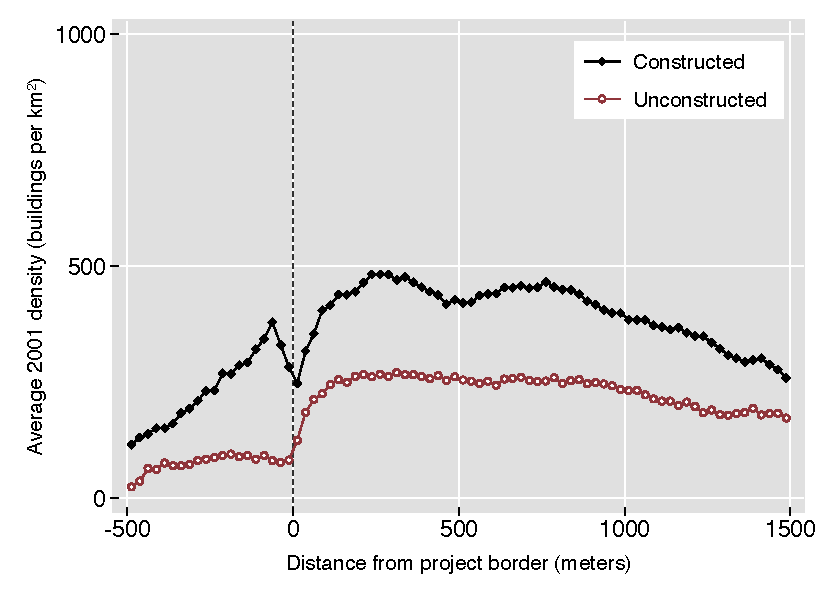
\includegraphics[width=\textwidth,trim={0.3cm .3cm 0.1cm 0cm}, clip=true]{figures/bblu_for_pre_means_4_spk.pdf}

        \end{subfigure}
        \hfill
        \begin{subfigure}[b]{0.48\textwidth}  
                    \caption[]%
            {{\footnotesize \textbf{All Projects} pre-period informal  raw data}}      
            \label{fig:preinf}
            \centering 
            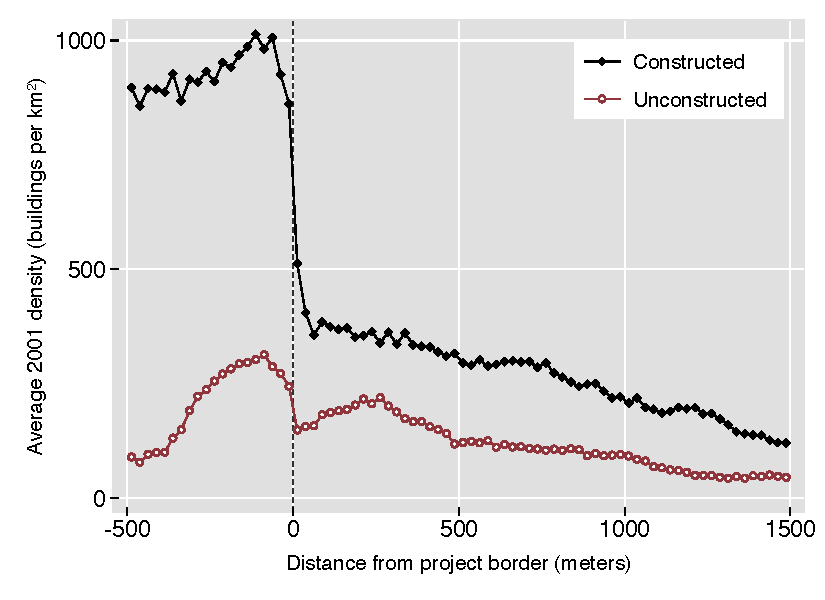
\includegraphics[width=\textwidth,trim={0.3cm .3cm 0.1cm 0cm}, clip=true]{figures/bblu_inf_pre_means_4_spk.pdf}

        \end{subfigure}
        \begin{subfigure}[b]{0.48\textwidth}
                    \caption[Network2]%
            {{\footnotesize \textbf{Greenfield} pre-period formal  raw data}}    
            \label{fig:prefor}
            \centering
            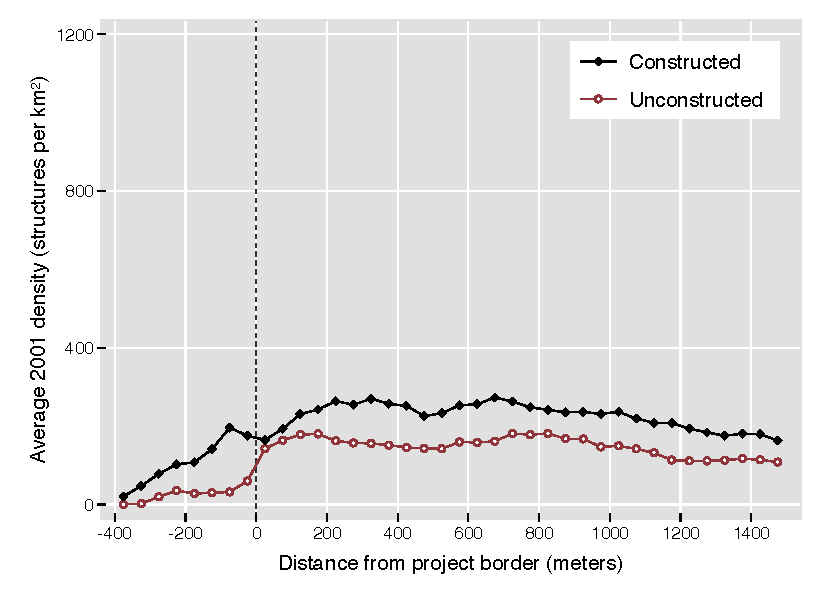
\includegraphics[width=\textwidth,trim={0.3cm .3cm 0.1cm 0cm}, clip=true]{figures/bblu_for_pre_means_4_1_spk.pdf}

        \end{subfigure}
        \hfill
        \begin{subfigure}[b]{0.48\textwidth}  
                    \caption[]%
            {{\footnotesize \textbf{Greenfield} pre-period informal  raw data}}     
            \label{fig:preinf}
            \centering 
            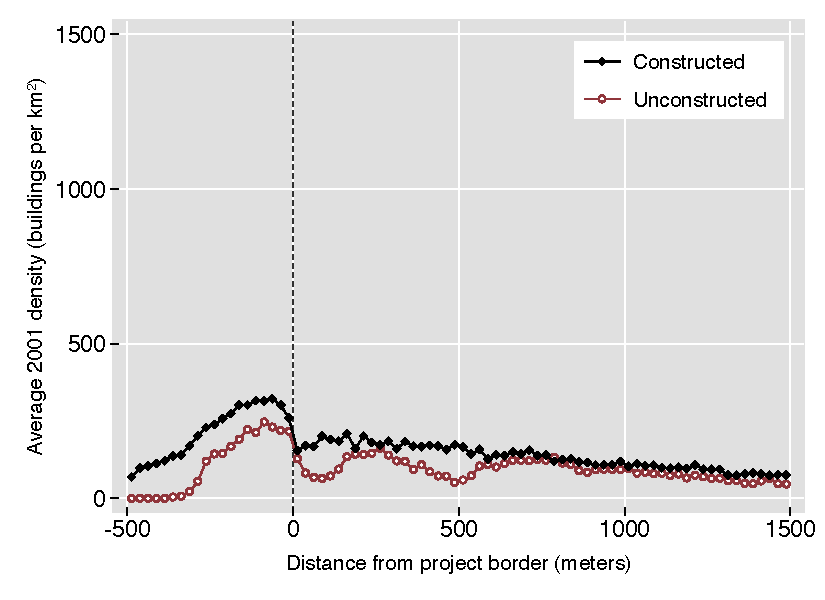
\includegraphics[width=\textwidth,trim={0.3cm .3cm 0.1cm 0cm}, clip=true]{figures/bblu_inf_pre_means_4_1_spk.pdf}

        \end{subfigure}
        \begin{subfigure}[b]{0.48\textwidth}
                    \caption[Network2]%
            {{\footnotesize \textbf{In-Situ} pre-period formal  raw data}}   
            \label{fig:prefor}
            \centering
            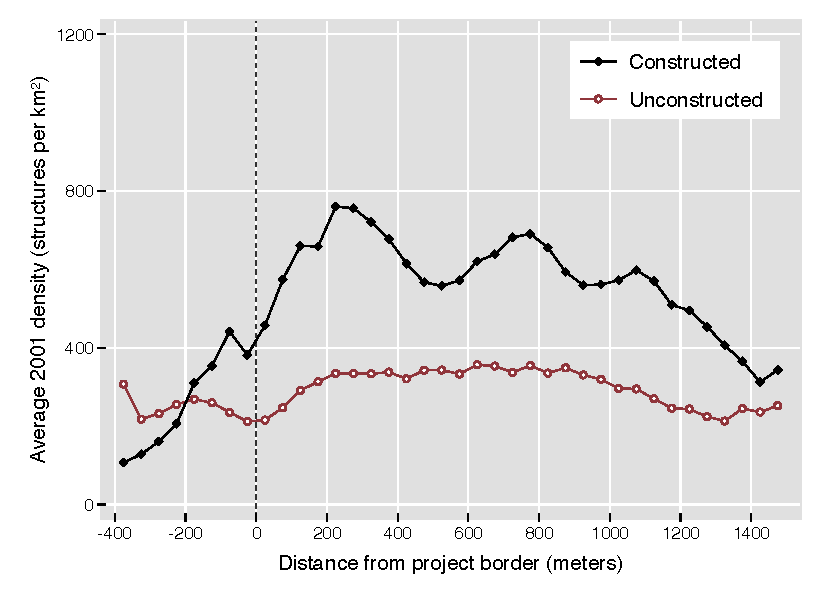
\includegraphics[width=\textwidth,trim={0.3cm .3cm 0.1cm 0cm}, clip=true]{figures/bblu_for_pre_means_4_2_spk.pdf}

        \end{subfigure}
        \hfill
        \begin{subfigure}[b]{0.48\textwidth}  
                    \caption[]%
            {{\footnotesize \textbf{In-Situ} pre-period informal  raw data}}     
            \label{fig:preinf}
            \centering 
            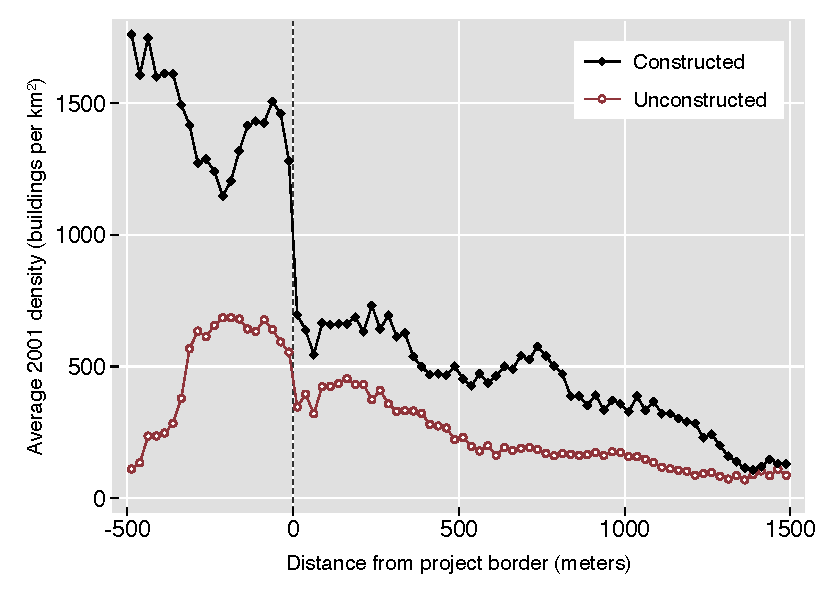
\includegraphics[width=\textwidth,trim={0.3cm .3cm 0.1cm 0cm}, clip=true]{figures/bblu_inf_pre_means_4_2_spk.pdf}

        \end{subfigure}
        \begin{subfigure}[b]{0.48\textwidth}
                    \caption[Network2]%
            {{\footnotesize \textbf{Other} pre-period formal  raw data}}   
            \label{fig:prefor}
            \centering
            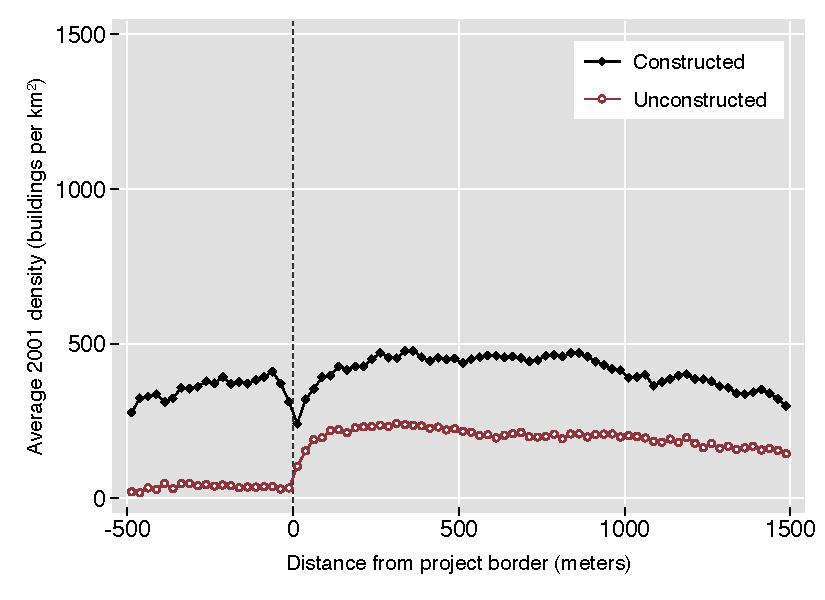
\includegraphics[width=\textwidth,trim={0.3cm .3cm 0.1cm 0cm}, clip=true]{figures/bblu_for_pre_means_4_3_spk.pdf}

        \end{subfigure}
        \hfill
        \begin{subfigure}[b]{0.48\textwidth}  
                    \caption[]%
            {{\footnotesize \textbf{Other} pre-period informal  raw data}}      
            \label{fig:preinf}
            \centering 
            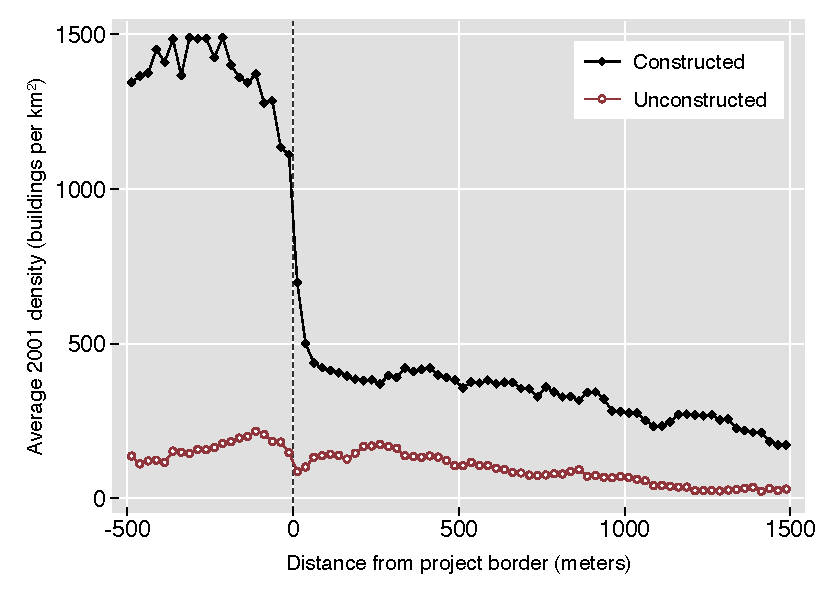
\includegraphics[width=\textwidth,trim={0.3cm .3cm 0.1cm 0cm}, clip=true]{figures/bblu_inf_pre_means_4_3_spk.pdf}

        \end{subfigure}
\end{figure*}








\begin{figure*}
        \centering
   %     \caption[ Pre-Period Housing Densities in Constructed and Unconstructed Projects Areas ]
  %      {\small Pre-Period Densities} 
        %\vspace{2mm}
        \begin{subfigure}[b]{0.48\textwidth}
            \caption[Network2]%
            {{\footnotesize \textbf{All Projects} changes formal raw data}}    
            \label{fig:prefor}
            \centering
            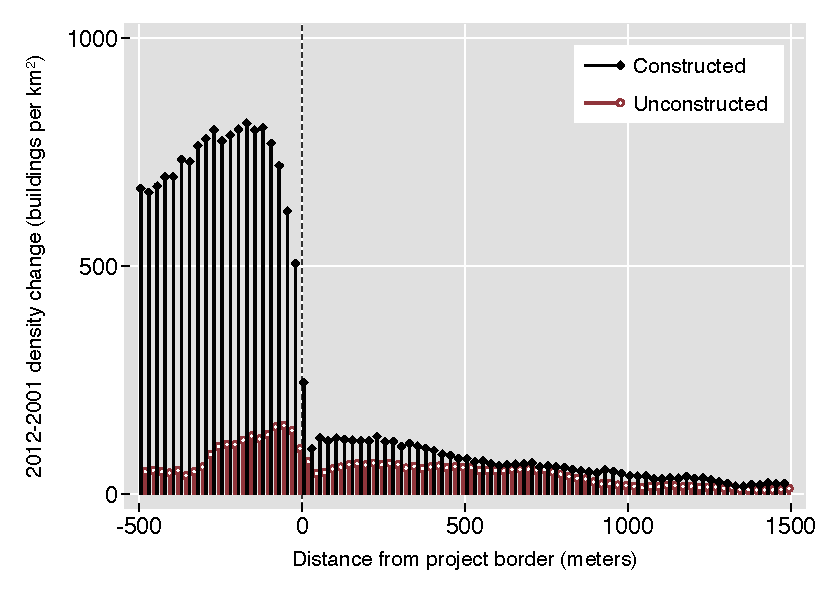
\includegraphics[width=\textwidth,trim={0.3cm .3cm 0.1cm 0cm}, clip=true]{figures/bblu_for_rawchanges_4_spk.pdf}

        \end{subfigure}
        \hfill
        \begin{subfigure}[b]{0.48\textwidth}  
                    \caption[]%
            {{\footnotesize \textbf{All Projects} changes informal  raw data}}      
            \label{fig:preinf}
            \centering 
            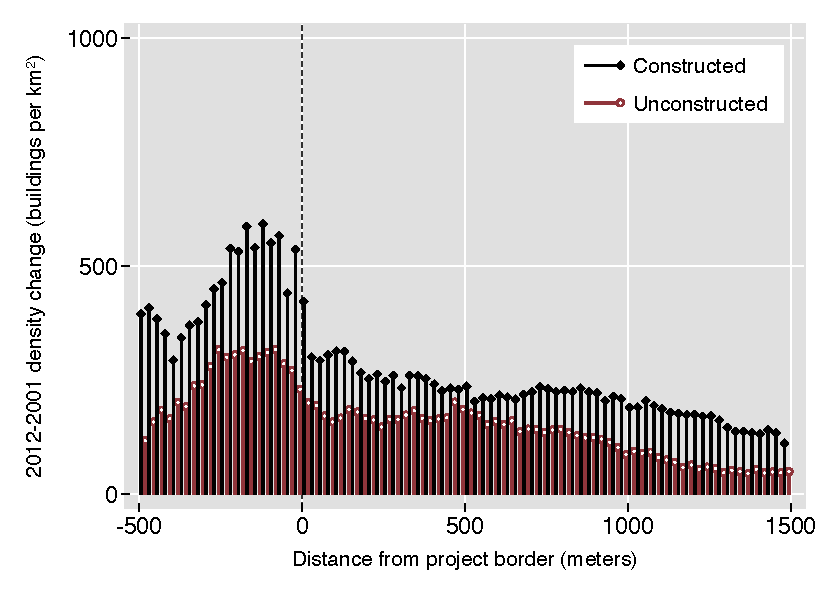
\includegraphics[width=\textwidth,trim={0.3cm .3cm 0.1cm 0cm}, clip=true]{figures/bblu_inf_rawchanges_4_spk.pdf}

        \end{subfigure}
        \begin{subfigure}[b]{0.48\textwidth}
                    \caption[Network2]%
            {{\footnotesize \textbf{Greenfield} changes formal  raw data}}    
            \label{fig:prefor}
            \centering
            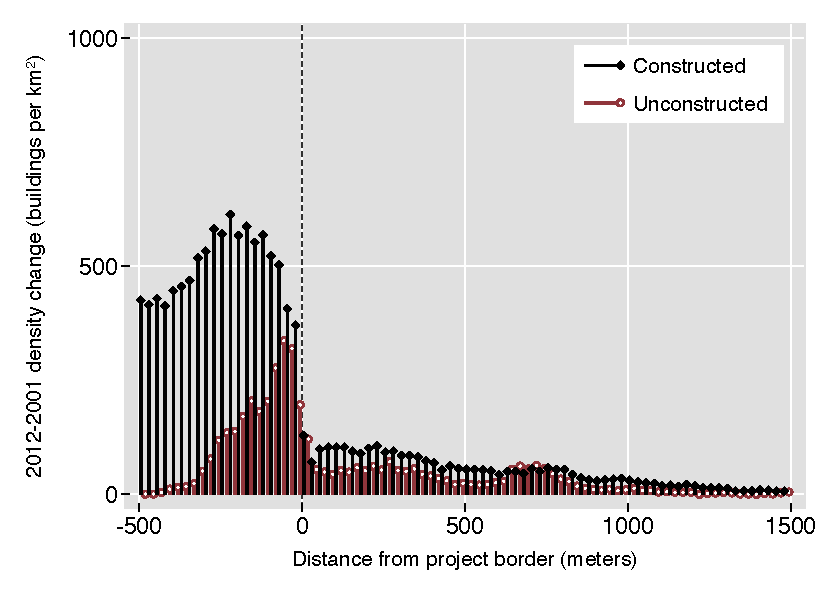
\includegraphics[width=\textwidth,trim={0.3cm .3cm 0.1cm 0cm}, clip=true]{figures/bblu_for_rawchanges_4_1_spk.pdf}

        \end{subfigure}
        \hfill
        \begin{subfigure}[b]{0.48\textwidth}  
                    \caption[]%
            {{\footnotesize \textbf{Greenfield} changes informal raw data }}     
            \label{fig:preinf}
            \centering 
            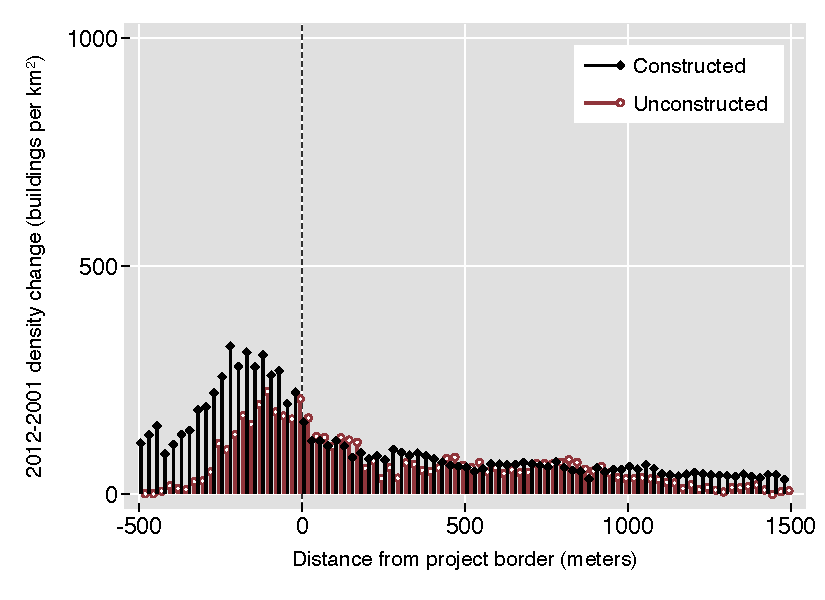
\includegraphics[width=\textwidth,trim={0.3cm .3cm 0.1cm 0cm}, clip=true]{figures/bblu_inf_rawchanges_4_1_spk.pdf}

        \end{subfigure}
        \begin{subfigure}[b]{0.48\textwidth}
                    \caption[Network2]%
            {{\footnotesize \textbf{In-Situ} changes formal raw data }}   
            \label{fig:prefor}
            \centering
            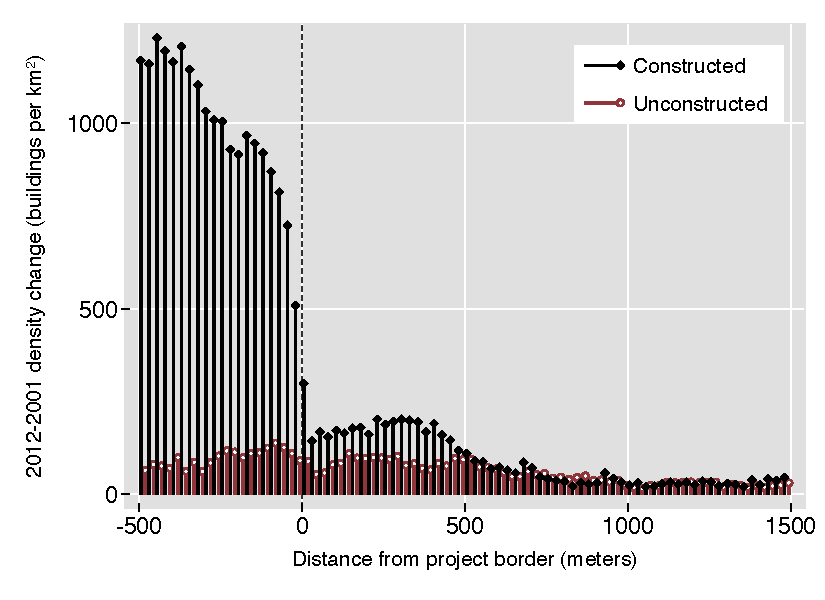
\includegraphics[width=\textwidth,trim={0.3cm .3cm 0.1cm 0cm}, clip=true]{figures/bblu_for_rawchanges_4_2_spk.pdf}

        \end{subfigure}
        \hfill
        \begin{subfigure}[b]{0.48\textwidth}  
                    \caption[]%
            {{\footnotesize \textbf{In-Situ} changes informal raw data }}     
            \label{fig:preinf}
            \centering 
            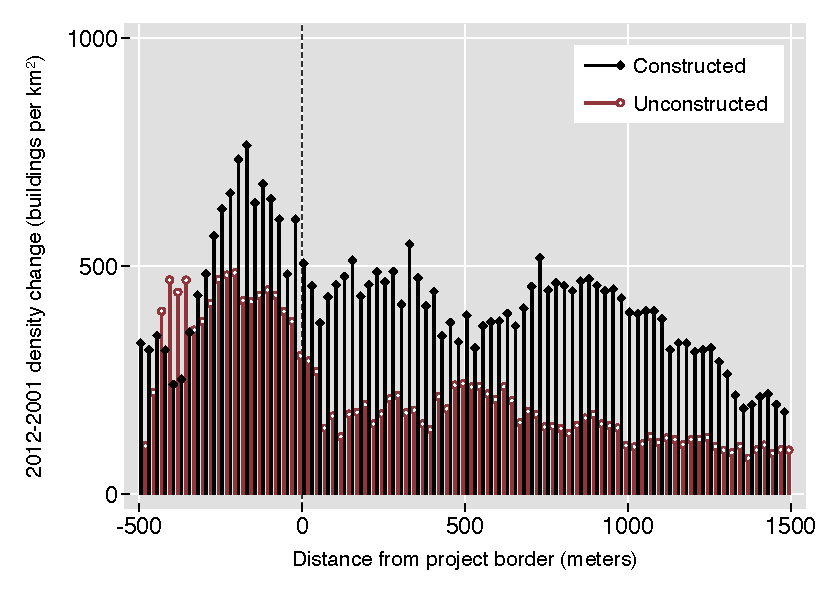
\includegraphics[width=\textwidth,trim={0.3cm .3cm 0.1cm 0cm}, clip=true]{figures/bblu_inf_rawchanges_4_2_spk.pdf}

        \end{subfigure}
        \begin{subfigure}[b]{0.48\textwidth}
                    \caption[Network2]%
            {{\footnotesize \textbf{Other} changes formal raw data}}   
            \label{fig:prefor}
            \centering
            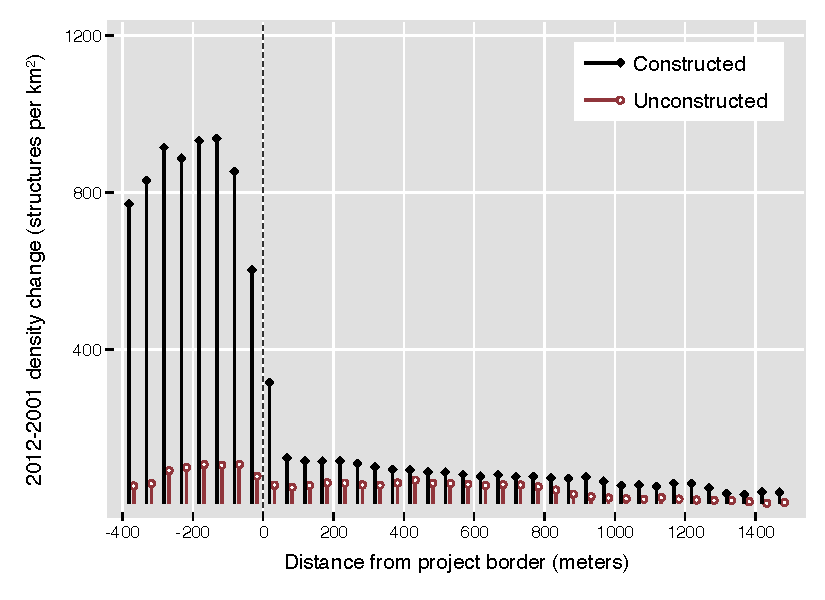
\includegraphics[width=\textwidth,trim={0.3cm .3cm 0.1cm 0cm}, clip=true]{figures/bblu_for_rawchanges_4_3_spk.pdf}

        \end{subfigure}
        \hfill
        \begin{subfigure}[b]{0.48\textwidth} 
                    \caption[]%
            {{\footnotesize \textbf{Other} changes informal  raw data}}      
            \label{fig:preinf} 
            \centering 
            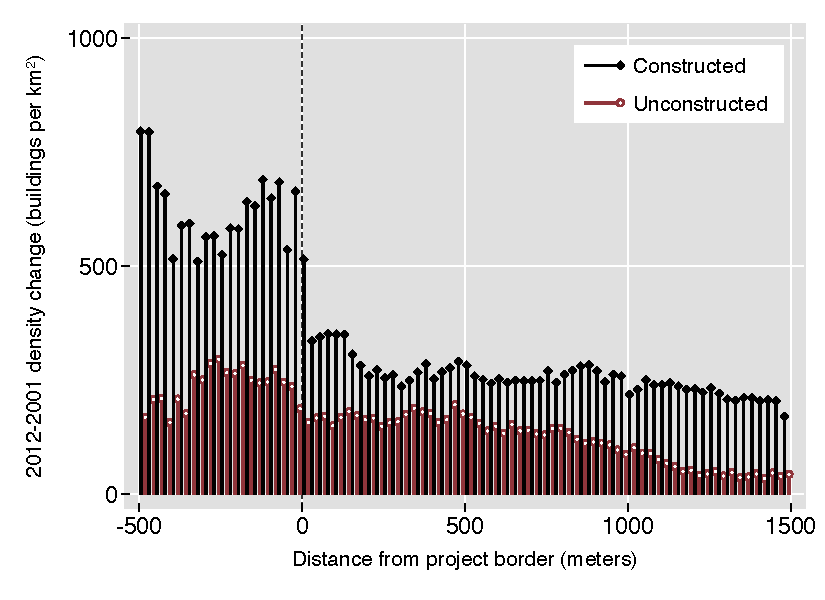
\includegraphics[width=\textwidth,trim={0.3cm .3cm 0.1cm 0cm}, clip=true]{figures/bblu_inf_rawchanges_4_3_spk.pdf}

        \end{subfigure}
\end{figure*}







\begin{table}
\caption{Building Density}
\begin{tabular}{lDDDDD}
\toprule
 & \small (1) & \small (2)  & \small (3) & \small (4) & \small (5) \\
 & Total & Formal  & Informal & Informal Bkyd. & Informal Non-Bkyd. \\ \midrule
\textbf{All Projects} \\inside project      &     798.586\textsuperscript{a}&     620.634\textsuperscript{a}&     177.952\textsuperscript{c}&     568.624\textsuperscript{a}&    -390.672\textsuperscript{a}\\
                    &   (140.082)                   &    (73.493)                   &    (95.550)                   &    (98.610)                   &    (80.861)                   \\[0.5em]
0-500m outside project &      48.071                   &      42.254\textsuperscript{b}&       5.817                   &      39.088                   &     -33.271                   \\
                    &    (38.845)                   &    (18.398)                   &    (33.441)                   &    (29.352)                   &    (22.649)                   \\[0.5em]
R$^2$               &       0.072                   &       0.050                   &       0.061                   &       0.049                   &       0.045                   \\

\midrule
\textbf{Greenfield} \\   inside project      &     479.700\textsuperscript{b}&     347.125\textsuperscript{b}&     132.575                   &     208.015\textsuperscript{b}&     -75.440                   \\
                    &   (201.670)                   &   (137.937)                   &    (90.025)                   &   (101.128)                   &    (64.406)                   \\[0.01em]
0-500m outside project &     -42.472                   &     -37.833                   &      -4.639                   &     -14.872                   &      10.233                   \\
                    &    (84.487)                   &    (49.952)                   &    (48.065)                   &    (34.612)                   &    (41.339)                   \\[0.8em] 
\textbf{In-Situ Upgrading} \\   inside project      &     921.187\textsuperscript{b}&     935.457\textsuperscript{a}&     -14.270                   &     827.893\textsuperscript{a}&    -842.163\textsuperscript{a}\\
                    &   (381.990)                   &   (157.961)                   &   (285.361)                   &   (264.315)                   &   (217.293)                   \\[0.01em]
0-500m outside project &     281.167\textsuperscript{c}&     191.798\textsuperscript{c}&      89.369                   &     143.355                   &     -53.986                   \\
                    &   (165.870)                   &    (99.793)                   &   (112.161)                   &   (115.769)                   &    (87.653)                   \\[0.8em]
\textbf{Other} \\   inside project      &     945.406\textsuperscript{a}&     685.781\textsuperscript{a}&     259.625\textsuperscript{c}&     695.491\textsuperscript{a}&    -435.866\textsuperscript{a}\\
                    &   (178.100)                   &    (78.228)                   &   (139.998)                   &   (117.367)                   &    (99.857)                   \\[0.01em]
0-500m outside project &      -3.350                   &      27.362                   &     -30.712                   &      15.646                   &     -46.358                   \\
                    &    (73.236)                   &    (32.053)                   &    (57.004)                   &    (46.598)                   &    (29.313)                   \\[0.8em]
Mean Outcome 2001   &      526.22                   &      261.56                   &      264.66                   &       96.43                   &      168.23                   \\
Mean Outcome 2011   &      838.62                   &      385.14                   &      453.48                   &      286.79                   &      166.69                   \\
R$^2$               &       0.114                   &       0.070                   &       0.102                   &       0.076                   &       0.073                   \\
N                   &   1,705,534                   &   1,705,534                   &   1,705,534                   &   1,705,534                   &   1,705,534                   \\

\bottomrule
\end{tabular}
\end{table}





\begin{table}[h!] 
\caption{Effect of Housing Projects on Socio-demographics}
\label{table:sorting}
\small
\centering
%\caption{Census Composition Estimates }
\vspace{-2mm}
\begin{tabular}{lDDDDD}
\toprule
& \small (1) & \small (2) & \small (3) & \small (4)& \small (5)\\
& \small Age & \small P.O.B. not Gauteng & \small Unemployed & \small Years of Education & \small Monthly Income \\ \midrule 
\textbf{All Projects} \\inside project      &       0.184                   &      -0.044                   &       0.012                   &       0.295\textsuperscript{b}&    1926.199\textsuperscript{a}\\
                    &     (0.377)                   &     (0.031)                   &     (0.019)                   &     (0.144)                   &   (533.707)                   \\[0.5em]
0-500m outside project &       0.062                   &       0.006                   &       0.003                   &       0.081                   &     765.829                   \\
                    &     (0.299)                   &     (0.020)                   &     (0.015)                   &     (0.096)                   &   (507.493)                   \\[0.5em]
R$^2$               &       0.181                   &       0.104                   &       0.196                   &       0.374                   &       0.171                   \\

\midrule
\textbf{Greenfield} \\   inside project      &      -2.194\textsuperscript{a}&       0.010                   &       0.085                   &      -0.679                   &     412.477                   \\
                    &     (0.629)                   &     (0.055)                   &     (0.054)                   &     (0.446)                   &  (1109.277)                   \\[0.01em]
0-500m outside project &      -1.225\textsuperscript{c}&       0.015                   &       0.078\textsuperscript{c}&      -0.324                   &    -914.047                   \\
                    &     (0.658)                   &     (0.066)                   &     (0.040)                   &     (0.228)                   &   (851.259)                   \\[0.8em] 
\textbf{In-Situ Upgrading} \\   inside project      &       0.326                   &      -0.119\textsuperscript{c}&       0.012                   &       0.289                   &    1438.091                   \\
                    &     (0.875)                   &     (0.066)                   &     (0.035)                   &     (0.251)                   &  (1413.506)                   \\[0.01em]
0-500m outside project &      -0.659                   &      -0.028                   &       0.022                   &       0.103                   &     386.747                   \\
                    &     (0.777)                   &     (0.056)                   &     (0.034)                   &     (0.261)                   &  (1329.296)                   \\[0.8em]
\textbf{Other} \\   inside project      &       0.714                   &       0.011                   &      -0.010                   &       0.534\textsuperscript{b}&    2766.503\textsuperscript{a}\\
                    &     (0.633)                   &     (0.044)                   &     (0.035)                   &     (0.219)                   &   (864.598)                   \\[0.01em]
0-500m outside project &       0.875                   &       0.022                   &      -0.038                   &       0.210                   &    1645.647\textsuperscript{b}\\
                    &     (0.565)                   &     (0.037)                   &     (0.028)                   &     (0.155)                   &   (800.367)                   \\[0.8em]
Mean Outcome 2001   &       27.30                   &        0.37                   &        0.47                   &        8.27                   &    2,477.01                   \\
Mean Outcome 2011   &       28.30                   &        0.43                   &        0.33                   &        9.68                   &    4,486.48                   \\
R$^2$               &       0.193                   &       0.136                   &       0.203                   &       0.389                   &       0.191                   \\
N                   &      12,734                   &      12,727                   &      12,724                   &      12,728                   &      12,724                   \\

\bottomrule
\multicolumn{6}{l}{\footnotesize Standard errors clustered at the project level in parenthesis. \textsuperscript{c} p$<$0.10, \textsuperscript{b} p$<$0.05, \textsuperscript{a} p$<$0.01  }\\
\multicolumn{6}{l}{\footnotesize P.O.B. means ``place of birth.''  Monthly income is in Rands.}
\end{tabular}
\end{table}








\begin{landscape}
{\footnotesize

\begin{table}[]
\small
\centering
\caption{Census Household-level Estimates }\label{table:censusestimates}
\vspace{-2mm}
\resizebox{.9\linewidth}{!}{
\begin{tabular}{lDDDDDDDD}
\toprule
 & \small (1) & \small (2)  & \small (3) & \small (4) & \small (5)  & \small (6)  & \small (7) & (8)\\
 & \small Flush Toilet & \small Water Indoors  & \small Electricity Cooking & \small Electricity Heating & \small Electricity Lighting  & \small Number of Rooms  & \small Household Size & Population Density\\ \midrule 
\textbf{All Projects} \\inside project      &       0.098                   &       0.199\textsuperscript{a}&       0.235\textsuperscript{a}&       0.169\textsuperscript{b}&       0.108                   &       0.325                   &       0.153                   &   -3959.188                   \\
                    &     (0.083)                   &     (0.050)                   &     (0.083)                   &     (0.079)                   &     (0.086)                   &     (0.203)                   &     (0.117)                   &  (2569.604)                   \\[0.5em]
0-500m outside project &      -0.040                   &       0.034                   &       0.012                   &       0.000                   &      -0.010                   &       0.121                   &       0.023                   &   -1933.915                   \\
                    &     (0.033)                   &     (0.034)                   &     (0.032)                   &     (0.035)                   &     (0.030)                   &     (0.141)                   &     (0.062)                   &  (1646.850)                   \\[0.5em]
R$^2$               &       0.101                   &       0.147                   &       0.185                   &       0.167                   &       0.100                   &       0.096                   &       0.094                   &       0.014                   \\

\midrule
\textbf{Greenfield} \\   inside project      &      -0.073                   &       0.092                   &       0.026                   &      -0.017                   &       0.026                   &      -0.010                   &       0.223                   &    6643.594\textsuperscript{c}\\
                    &     (0.159)                   &     (0.124)                   &     (0.127)                   &     (0.137)                   &     (0.137)                   &     (0.296)                   &     (0.142)                   &  (3405.909)                   \\[0.01em]
0-500m outside project &      -0.102\textsuperscript{c}&      -0.064                   &      -0.043                   &      -0.022                   &       0.028                   &      -0.249                   &       0.152                   &    5774.084                   \\
                    &     (0.060)                   &     (0.097)                   &     (0.066)                   &     (0.068)                   &     (0.043)                   &     (0.355)                   &     (0.131)                   &  (4503.950)                   \\[0.8em] 
\textbf{In-Situ Upgrading} \\   inside project      &       0.367\textsuperscript{b}&       0.187\textsuperscript{c}&       0.299\textsuperscript{b}&       0.267\textsuperscript{b}&       0.191                   &       0.797\textsuperscript{b}&       0.482\textsuperscript{b}&   -9431.142                   \\
                    &     (0.153)                   &     (0.112)                   &     (0.130)                   &     (0.124)                   &     (0.124)                   &     (0.378)                   &     (0.241)                   &  (5887.945)                   \\[0.01em]
0-500m outside project &      -0.000                   &      -0.006                   &       0.036                   &       0.023                   &       0.007                   &      -0.057                   &       0.147                   &   -2842.097                   \\
                    &     (0.084)                   &     (0.097)                   &     (0.072)                   &     (0.081)                   &     (0.067)                   &     (0.371)                   &     (0.139)                   &  (3666.322)                   \\[0.8em]
\textbf{Other} \\   inside project      &      -0.051                   &       0.239\textsuperscript{a}&       0.188                   &       0.111                   &       0.028                   &       0.114                   &      -0.123                   &   -4628.290                   \\
                    &     (0.107)                   &     (0.077)                   &     (0.114)                   &     (0.106)                   &     (0.125)                   &     (0.338)                   &     (0.153)                   &  (3540.290)                   \\[0.01em]
0-500m outside project &      -0.040                   &       0.094                   &       0.008                   &      -0.008                   &      -0.028                   &       0.369                   &      -0.091                   &   -4418.420                   \\
                    &     (0.041)                   &     (0.058)                   &     (0.044)                   &     (0.046)                   &     (0.043)                   &     (0.258)                   &     (0.102)                   &  (3390.889)                   \\[0.8em]
Mean Outcome 2001   &        0.79                   &        0.35                   &        0.66                   &        0.62                   &        0.77                   &        3.30                   &        3.51                   &    8,566.83                   \\
Mean Outcome 2011   &        0.83                   &        0.54                   &        0.81                   &        0.72                   &        0.82                   &        3.56                   &        3.18                   &    9,823.82                   \\
R$^2$               &       0.111                   &       0.170                   &       0.202                   &       0.186                   &       0.120                   &       0.109                   &       0.107                   &       0.051                   \\
N                   &      12,732                   &      12,732                   &      12,732                   &      12,732                   &      12,732                   &      12,709                   &      12,730                   &      12,734                   \\

\bottomrule
\multicolumn{9}{l}{\footnotesize All regressions include 3km grid Fixed-Effects. Standard errors clustered at the project level in parenthesis. \textsuperscript{c} p$<$0.10,\textsuperscript{b} p$<$0.05,\textsuperscript{a} p$<$0.01 }
\end{tabular}
}
\end{table}

}
\end{landscape}




\begin{table}
\small
\centering
\caption{Triple Difference Estimates on Log-Prices}\label{table:priceDDD_het}
\vspace{-2mm}
\begin{tabular}{lCC}
\toprule
 & \small (1) & \small (2)  \\ \midrule 
 \textbf{All Projects} \\
 inside project      &       0.331                   &       0.336                   \\
                    &     (0.530)                   &     (0.530)                   \\[0.5em]
0-500m outside project &      -0.178                   &      -0.177                   \\
                    &     (0.141)                   &     (0.141)                   \\[0.5em]
Lot Size Controls   &                               &  \checkmark                   \\
r2                  &        0.18                   &        0.18                   \\
N                   &      67,751                   &      67,751                   \\

 \midrule
\textbf{Greenfield} \\   inside project      &       0.414                   &       0.407                   \\
                    &     (0.409)                   &     (0.408)                   \\[0.01em]
0-500m outside project &      -0.107                   &      -0.108                   \\
                    &     (0.218)                   &     (0.218)                   \\[0.8em]
\textbf{In-Situ Upgrading} \\   inside project      &       0.358                   &       0.374                   \\
                    &     (0.559)                   &     (0.563)                   \\[0.01em]
0-500m outside project &      -0.170                   &      -0.168                   \\
                    &     (0.324)                   &     (0.324)                   \\[0.8em]
\textbf{Other} \\   inside project      &      -0.800                   &      -0.799                   \\
                    &     (0.524)                   &     (0.524)                   \\[0.01em]
0-500m outside project &      -0.225                   &      -0.224                   \\
                    &     (0.198)                   &     (0.199)                   \\[0.8em]
Lot Size Controls   &                               &  \checkmark                   \\
r2                  &        0.21                   &        0.22                   \\
N                   &      67,751                   &      67,751                   \\

\bottomrule
\multicolumn{3}{l}{\footnotesize Standard errors clustered at the project level in parenthesis.} \\
\multicolumn{3}{l}{ \textsuperscript{c} p$<$0.10,\textsuperscript{b} p$<$0.05,\textsuperscript{a} p$<$0.01 }
\end{tabular}
\end{table} 

% \begin{figure}
% 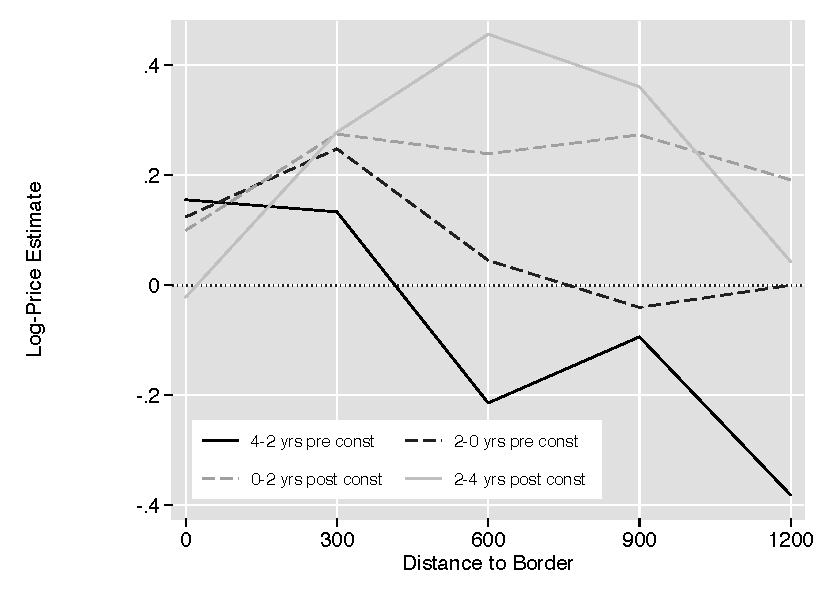
\includegraphics{figures/price_to_event_30.pdf}
% \end{figure}


\end{document}


